\documentclass[oneside]{book}
\usepackage{epsfig,graphicx} % Required for inserting images
\usepackage{amsmath}
\usepackage{amsthm}
\usepackage{amssymb}
\usepackage{subcaption}
\usepackage[spanish,mexico]{babel}
\usepackage[bookmarksopen]{hyperref}
\usepackage[utf8]{inputenc}
\usepackage{array}
\usepackage{listings} %Soporte para código
\usepackage[left=2cm,right=2cm,top=1.8cm,bottom=2.3cm]{geometry}
%\usepackage{schemata}
% ---definición de los paquetes--
\usepackage{fancyhdr}            % Permits header customization. See header section below.
\fancypagestyle{plain}{
\lhead{}
\fancyhead[R]{\thepage}
\fancyhead[L]{}
\renewcommand{\headrulewidth}{0pt}
\fancyfoot{}
}
\pagestyle{fancy}
\fancyhead[R]{\thepage}
\fancyhead[L]{}
\title{Tarea 02: Lógica Proposicional}
\author{Ramírez Mendoza Joaquín Rodrigo\\
Villalobos Juárez Gontran Eliut\\
Treviño Puebla Héctor Jerome}
\date{\today}
% ---Inicio de la portada
\begin{document}
\begin{titlepage}
	\begin{minipage}{3cm}
		\begin{center}
			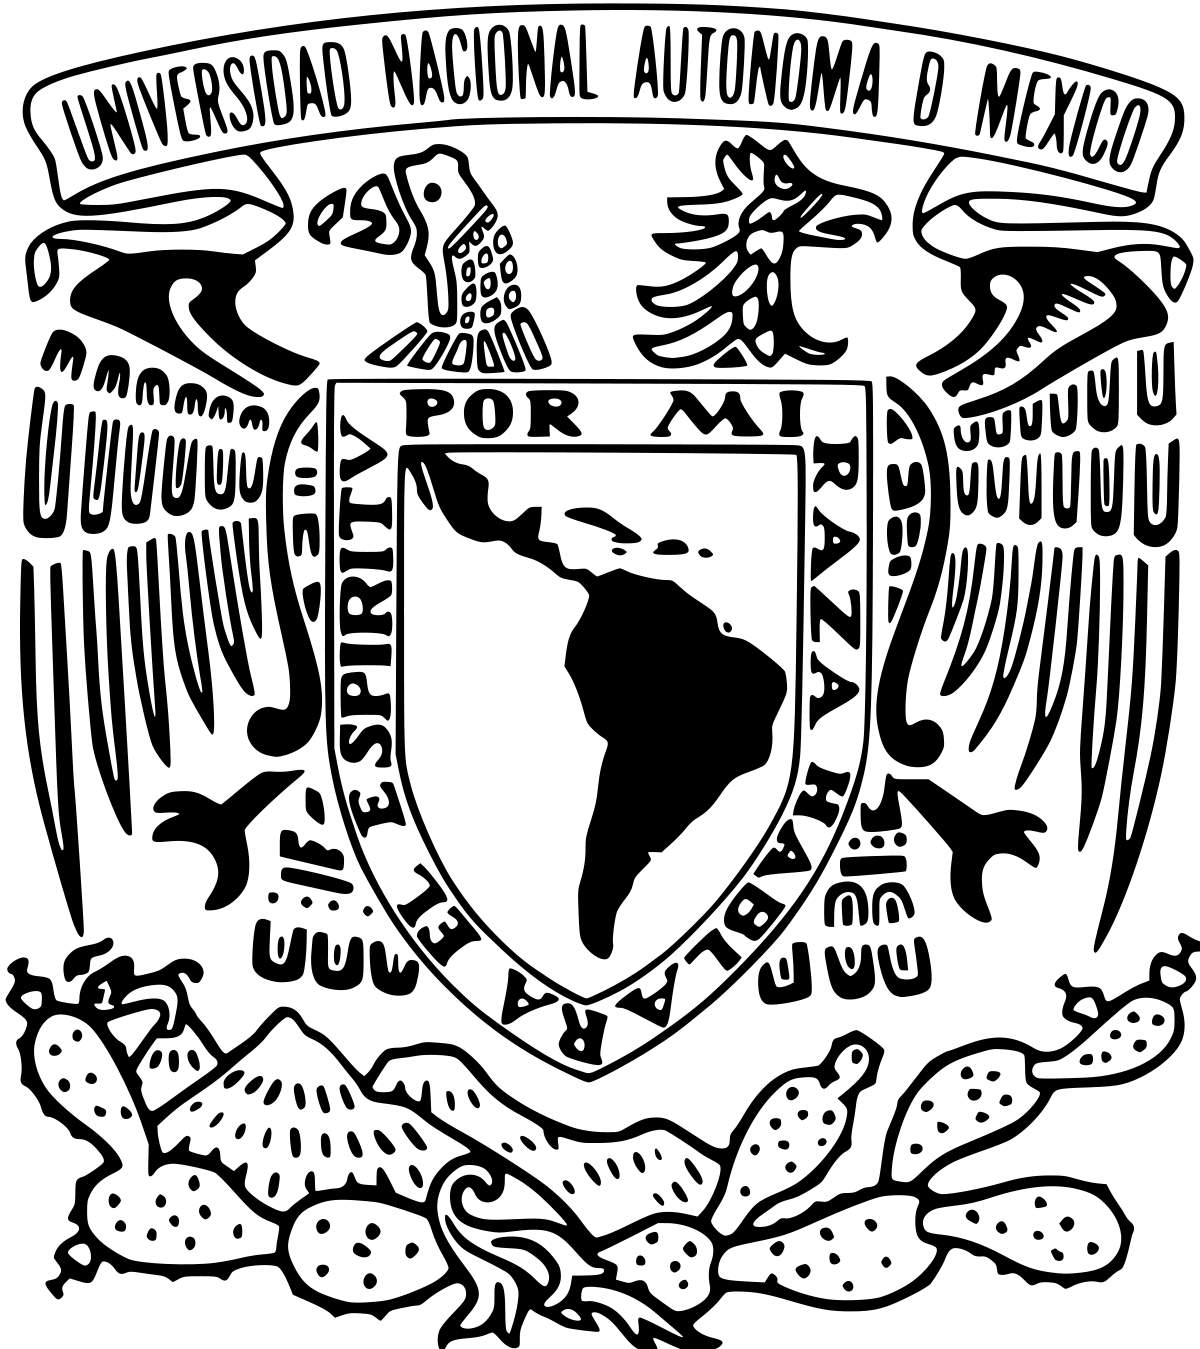
\includegraphics[height = 0.14\textheight]{recursos/Logo_UNAM.png}\par
		\end{center}
	\end{minipage}\hfill
	\begin{minipage}{10cm}

	\end{minipage}\hfill
	\begin{minipage}{3cm}
		\begin{center}
			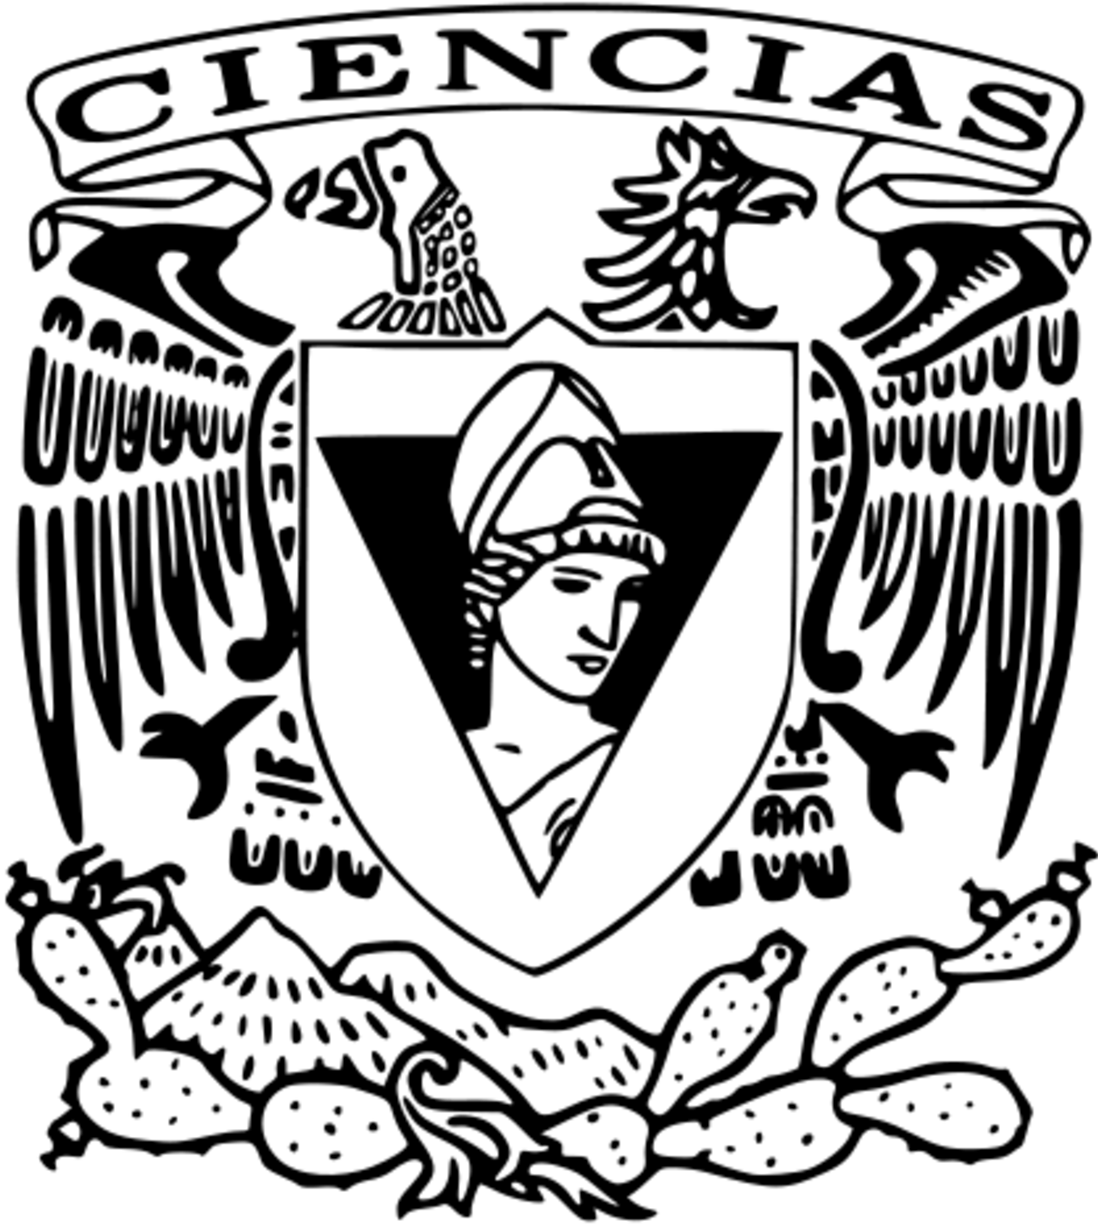
\includegraphics[height = 0.14\textheight]{recursos/Logo_FC.png}\par
		\end{center}
	\end{minipage}
	\centering
	\vspace{1cm}

	{\bfseries\LARGE Universidad Nacional Autónoma de México \par}

	\vspace{1cm}
	{\scshape\Large Facultad de Ciencias \par}
	\vspace{1cm}
	{\scshape\Large Estructuras Discretas \par}
	\vspace{1cm}
	{\scshape\Large Licenciatura en Ciencias de la Computación \par}
	\vspace{1cm}
	{\scshape\Huge Tarea 02: Lógica Proposicional.  \par}
	\vspace{3cm}
	{\itshape\Large Segundo Parcial \par}
	\vfill
	{\Large Autores: \par}
	{\Large Ramírez Mendoza Joaquín Rodrigo \par}
	{\Large Villalobos Juárez Gontran Eliut\par}
	{\Large Treviño Puebla Héctor Jerome \par}
	\vfill
	{\Large Octubre 2024 \par}
\end{titlepage}
% ---Fin de la portada de la portada
\maketitle

% Introducir aquí sus capítulos
% ------∨∨∨∨∨∨∨∨∨∨∨∨∨∨∨--------
\noindent\textbf{1. De las siguientes expresiones, identificar las proposiciones atomicas y los conectores lógicos. Traducir de lenguaje natural a lenguaje lógico:}

\begin{multicols}{2}
	\begin{enumerate}[label=\alph*)]
		\item Penélope es griega.
		\item Alonso Quijano no está cuerdo.
		\item Si Juan fue al cine, seguro que Lupe también.
		\item Melibea no está triste, porque cursó Estructuras Discretas.
		\item Juan come y bebe.
		\item Cuando María estudia, no reprueba los exámenes.
		\item Armin no fuma ni bebe.
		\item Juana juega fútbol, pero no baloncesto.
	\end{enumerate}
\end{multicols}

\textbf{a)}$p$ = \newpage
\end{document}